\subsubsection{\ac{REST} Allgemein}
\label{sec:RESTAllgemein}

Im Folgenden soll die Technologie \ac{REST} vorgestellt werden.
Zunächst wird \ac{REST} etwas genauer anhand von Beispielen erläutert.
Anschließend werden die Vor- und Nachteile dargestellt, sowie die Kernpunkte erläutert.

\subsubsection{\ac{REST} Beispiel}
\label{sec:RESTBeispiel}

Um Daten von einer \ac{REST}-Schnittstelle zu bekommen, werden die \ac{HTTP}-Methoden in Verbindung mit einer entsprechenden \ac{URI} verwendet. Im Folgenden wird dies anhand einiger Beispiele gezeigt:

GET /resources/
Liefert eine Liste aller Ressourcen.

GET /resources/4
Liefert die Ressource mit ID = 4.

POST /resources/
Legt eine neue Ressource an.

PUT /resources/4
Aktualisiert die Ressource mit ID = 4.

DELETE /resources/4
Löscht die Ressource mit ID = 4.

Einen tieferen Einblick, wann und wie die Methoden genutzt werden, wird in Abschnitt \ref{sec:RESTHTTP} gegeben.

\subsubsection{Ressourcen}
\label{sec:RESTRessourcen}

Im Folgenden werden Datensätze als Ressourcen bezeichnet. Dabei kann man die Ressourcen weiter unterteilen:

–	Primärressourcen: Unter Primärressourcen fallen komplette, vollständige Ressourcen

–	Subressourcen: Subressourcen sind Teile von Primärressourcen

–	Listen: Eine Liste umfasst eine Menge von Ressourcen

–	Filter: Anwendung von Filterkriterien auf Listen

–	Paginierung: begrenzte Datenmenge

–	Projektionen: Teil der Informationen einer Primärressource

–	Aggregationen: Zusammenfassung mehrerer Ressourcen

\subsubsection{Merkmale}
\label{sec:RESTMerkmale}

Die Kommunikation erfolgt auf Abruf. Der Client ist aktiv und fordert vom passiven Server eine Repräsentation an, bzw. modifiziert eine Ressource. Ressourcen, die Objekte der Anwendung, besitzen eine ihnen zugeordnete \ac{URI}, mit der sie adressiert werden können. Die Repräsentation einer Ressource kann als Dokument vom Client angefordert werden. Repräsentationen können auf weitere Ressourcen verweisen, die ihrerseits wieder Repräsentationen liefern, die wiederum auf Ressourcen verweisen können. Der Server verfolgt keinen Clientstatus. Jede Anfrage an den Server muss alle Informationen beinhalten, die zum Interpretieren der Anfrage notwendig sind. Caches werden unterstützt. Der Server kann seine Antwort als cache-fähig oder nicht cache-fähig kennzeichnen.

Repräsentationen:

Um die Ressourcen darzustellen, werden in \ac{REST} mehrere Repräsentationen der Ressourcen genutzt. Dies entsteht aus der Intention heraus, dass aufgrund der unterschiedlichen Repräsentationen unterschiedliche Anforderungen der Clients bedient werden können. So kann zum Beispiel die \ac{HTML} Repräsentation für einen Webbrowser genutzt werden, während eine \ac{JSON} Repräsentation für eine Clientapplikation genutzt wird.

\subsubsection{Nutzung von \ac{HTTP}}
\label{sec:RESTHTTP}


Um auf eine Ressource zuzugreifen wird das \ac{HTTP}-Protokoll verwendet. Je nachdem, welche Verwendung die Ressourcen finden, werden geeignete \ac{HTTP}-Methoden verwendet. Die häufigsten Verwendeten Methoden sind dabei GET, POST, PUT und DELETE. Per GET werden Daten geladen; POST hat mehrere Einsatzgebiete. Häufig wird dadurch eine neuer Datensatz angelegt, oder mehrere Datensätzen aktualisiert. PUT aktualisiert einen bestimmten Datensatz und DELETE löscht einen Datensatz. Dabei müssen sinnvolle Statuscodes zurückgegeben werden. Zusätzlich gibt es noch die Methoden PATCH, HEAD und OPTIONS. Auf diese wird jedoch nicht weiter eingegangen, da diese eine vergleichsweise geringe Bedeutung bei einer \ac{REST}-Schnittstelle haben. Bei der Implementierung ist unbedingt zu beachten die Methoden idempotent zu gestalten, d.h. Ein mehrmaliges Aufrufen derselben Methode wirkt sich nicht anders aus, als ein einmaliger Aufruf. Einzige Ausnahme dabei ist die POST-Methode. Das Prinzip von \ac{REST} ist, Ressourcen von einem Zustand in den nächsten Zustand zu überführen.

\subsubsection{Statuscodes}
\label{sec:RESTStatuscodes}

Folgende Tabelle zeigt die allgemeine Bedeutung der unterschiedlichen Statuscodes

\begin{table}[!h]
	\begin{tabular}{ | l | l | }
		\hline
		Statuscode & Bedeutung \\ \hline
		1xx & Informationen \\ \hline
		2xx & Erfolgreiche Operationen \\ \hline
		3xx & Umleitung \\ \hline
		4xx & Client-Fehler \\ \hline
		5xx & Server-Fehler \\ \hline
	\end{tabular}
	\caption{Statuscodes}
\end{table}


\subsubsection{URI-Design}
\label{sec:RESTURI-Design}

Eine \ac{URL} lokalisiert eine Ressource, wobei eine \ac{URI} sie identifiziert. Lokalisierung kann dabei auch zur Identifizierung führen.
Eine \ac{URL} ist also immer eine \ac{URI}. Im Umkehrschluss kann eine \ac{URI} eine \ac{URL} sein, muss es
aber nicht.

Möchte man \ac{REST} in einem Satz definieren, dann ergibt sich: „Eine eigene URI für jedes Informationselement.“ (vgl. \cite{.j}\cite{Tilkov.2015b})

An diesem Satz sollte man sich auch beim \ac{URI}-Design halten. Ressourcen können so durch
ihre \ac{URI} eindeutig identifiziert werden. Dabei sollen diese so konstruiert werden, dass man
bereits aus der \ac{URI} alleine lesen kann, was für eine Ressource dahinter steckt. Eine \ac{URI} zeigt
auf eine Ressource, aber diese kann über mehrere \ac{URI}s angesprochen werden.
Die verschiedenen Ressourcenarten können auf folgende \ac{URI}-Strukturen abgebildet werden (vgl. Kapitel \ref{sec:RESTRessourcen}): 

–	Liste: /resources/:	Man bekommt mehrere Ressourcen gleicher Art

–	Primärressource: /resources/1:	Man bekommt genau eine unabhängige Ressource

–	Sekundärressource: /resources/subresources/1:	Man bekommt genau eine von einer anderen Ressource abhängige Ressource

–	Filter: /resources?name=a oder /resources/name=a : Man bekommt mehrere Ressourcen gleicher Art, die mit bestimmten Parametern gefiltert werden.

\subsubsection{HATEOAS}
\label{sec:RESTHATEOAS}

HATEOAS ist ein wichtiges Prinzip, welches von vielen selbsternannten \ac{REST}-Schnittstellen
nicht implementiert wird. Dieses Akronym beschreibt, dass die Schnittstelle über Hypertext
beziehungsweise Hypermedia angetrieben wird. Genauer gesagt, sollen durch den Aufruf
der Haupt-\ac{URI} alle Funktionalitäten als Hyperlinks unter Angabe der jeweiligen Beziehung
zugreifbar sein. Die Schnittstelle dokumentiert sich sozusagen selbst.
In seiner im Jahre 2000 verfassten Dissertation “Architectural Styles and the Design of
Network-based Software Architectures”, definiert Roy Fielding die \ac{REST}-Architektur. Dabei
geht er unter anderem auf Ressourcen und \ac{HTTP} ein. Als wichtigen Punkt sieht Fielding
jedoch auch die Verwendung von Hypermedia und die Verlinkung zwischen verwandten Ressourcen.
In 2008 verdeutlicht Fielding anhand eines Blogeintrags seinen Standpunkt zu \ac{REST}ful API's...
“If the engine of application state (and hence the API) is not being driven by hypertext, then
it cannot be RESTful and cannot be a REST API. Period. Is there some broken manual
somewhere that needs to be fixed?” – \cite{.19.03.2017}

Damit will er sagen, dass Schnittstellen, welche nicht über Hypertext gesteuert werden, auch
keine \ac{REST}-Schnittstellen sind, sondern ganz normale \ac{RPC}-Schnittstellen.
Um dieses Prinzip zu verdeutlichen wird anhand Abbildung 3 das Richardson Maturity Model
veranschaulicht.
 
\begin{figure}[!htb]
	\centering
	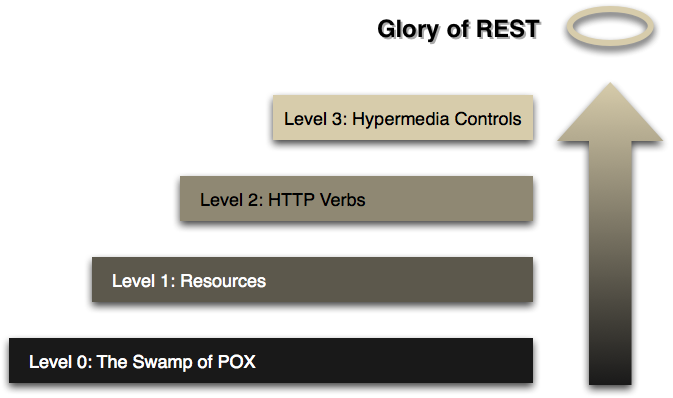
\includegraphics[scale=0.5]{hateoas.png}
	\caption[Richardson Maturity Model]{Richardson Maturity Model,\\ Quelle: https://martinfowler.com/articles/images/richardsonMaturityModel/ overview.png}
\end{figure}
 


Das Richardson Maturity Model unterteilt die \ac{REST}-Architektur in vier Stufen. Eine echte
\ac{REST}-Schnittstelle implementiert dabei alle vier Stufen. Doch gerade die letzte Stufe wird oft
nicht implementiert, da sie eine gewisse Komplexität birgt.

LEVEL 0 sagt lediglich aus, dass \ac{HTTP} als Transportprotokoll für \ac{RPC}-Aufrufe genutzt wird.
Die Kommunikation findet über eine einzige \ac{URI} statt.

LEVEL 1 sagt aus, dass jede Ressource eine eigene \ac{URI} hat.

In LEVEL 2 werden die bereits vorgestellten \ac{HTTP}-Methoden verwendet.

In der letzten Stufe, LEVEL 3, kristallisieren sich die Unterschiede zwischen richtigen \ac{REST}-
Services und solchen, die es gerne sein wollen, heraus. Durch den Einsatz von Hypermedia sollen alle
Ressourcen miteinander verknüpft werden. Dabei soll beim Aufruf der Haupt-\ac{URI} alle
möglichen Aufrufe zurückgegeben werden. Folgende Tabelle soll die Vor- und Nachteile von
HATEOAS verdeutlichen.
\newline

\begin{table}[H]
	\begin{tabular}{ | p{7cm} | p{7cm} | }	
		\hline	
		Vorteile & Nachteile \\  \hline	
		Entkopplung von Client und Server, da sich der Client nicht anpassen muss,
		wenn sich serverseitige Änderungen ergeben & 
		Findet relativ geringe Anwendung	 \\ \hline
		Transparenz von Änderungen in der Ressourcenverteilung: 
		Client kann Links folgen ohne die genaue Serverinfrastruktur zu kennen 
		& Steigert die Komplexität der Implementierung \\ \hline
		Serverseitig steuerbarer Anwendungsfluss: Server teilt mit, welche Aktionen möglich sind. 
		Der Client kann sich dynamisch danach richten.
		 & Bei Erweiterung der Schnittstelle müssen natürlich überall Anpassungen gemacht werden. \\ \hline
		Selbstbeschreibende API &  \\ \hline
	\end{tabular}
	\caption{Vorteile und Nachteile des Richardson Maturity Model}
\end{table}

Dass HATEOAS einen gewissen Nutzen bringt ist nicht abzustreiten, jedoch müssen diese mit den Kosten verglichen werden. Der Aufwand kann den Nutzen deutlich überwiegen, da macht es natürlich keinen Sinn dieses Prinzip anzuwenden. Dies ist vor allem bei kleineren internen Projekten, die nicht zur öffentlichen Verwendung gedacht sind, der Fall. Möchte man aber dem \ac{REST}-Prinzip hundertprozentig folgen, so muss HATEOAS implementiert werden.
